\section{Partitioning \java{} Applications}
\label{sec:civet:background}

%This section discusses the security features of  \sgx{}, and the challenges faced by developers that
%wish to use \sgx{} for partitioned \java{} applications.
%the key challenges developers face when trying to manually partition applications using a technology such as \sgx{}.
%discuss the programming models and threats to security of \sgx{} enclaves.

%\subsection{Security Concerns on SGX Enclaves}




%The rest of this subsection outlines several pitfalls in partitioning an application for SGX.



%\paragraph{Side Channels and Denial-of-Service.}
%In the current \sgx{} design, side channels are a significant concern, and are out of the scope of this paper.
%A controlled channel attack~\fixmedp{cite} can single step enclave execution by inducing page faults
%in the enclave.  \sysname{} does not specifically defend against side channel attacks,
%and we expect that any solution to this problem involves redesigning the %division of labor in virtual
%memory management for enclaves.

%Similarly, there is no guarantee that a compromised application will ever %enter
%an enclave.  Denial-of-service attacks are out of scope for this paper.

%% \paragraph{Writes outside of the enclave.}
%% However, the security of SGX enclaves is founded on trusting the code running inside the enclave.
%% SGX allows the trusted code to read and write data structures 
%% outside of the enclave.  Thus, it is easy for a developer to inadvertently write
%% code that discloses a secret, say by using a library that memoizes intermediate results to the untrusted heap.
%% A fundamental requirement is that developers must be able to reason about (or assert)
%% what code can and can't access data {\em outside} of the enclave.
%% \fixmedp{Can we say anything about whether such tools exist before Civet?}

%% %\fixmedp{Do I recall correctly that you can easily write to data outside of the enclave?  If so, this seems like something easy to get wrong, especially 
%% %if a library memoizes intermediate results.  The developer needs to be able to tell 
%% %Unless I am full of shit, can we paragraph-ize this fixme?

%% \paragraph{Vulnerabilities in the isolated applications.} 
%% One of the major threats to enclave security is the vulnerabilities in the isolated code,
%% such as memory corruption bugs,
%% control flow or information flows, semantic bugs, and so forth. 
%% %Moreover, although \sgx{} code integrity guarantees make enclaves resistant to code injection,
%% %an attacker may still manipulate control flow using code-reuse attacks~\citep{code-reuse-attacks}.
%% Moreover, recent research~\citep{hudata} shows that even with control flow integrity,
%% attackers can still manipulate the execution to leak the secrets through information flow.



%%% \sgx{} also proves the integrity of loaded binaries to remote trusted entities
%%% using mutual attestation based on a symmetric key generated from the measurements of communicating entities.
%%% \sgx{} usage model mostly involve the launched enclave mutually attesting the trusted host
%%% to obtain provisioning of security-sensitive information
%%% through a trusted channel. Such an execution model leverages resources such as CPU and DRAM from vulnerable untrusted \sgx{}-enabled hosts owned by cloud providers
%%% by extending the trust from
%%% the hosts owned and trusted by the clients or service providers.
%%% For instance, \sgx{} can isolate the decoder engine in an enclave
%%% after authenticating the customers to enforce Digital Right Management (DRM) even if the digital data is hosted on an untrusted cloud server.

%Use cases of \sgx{} mostly involve the launched enclave
%retrieving a cryptographically signed attestation from the processor,
%to exchange security critical information with remote servers through secured channels.
%The effect is equivalent to expanding the trusted space from remote servers
%to the local end, to harness local resources such as CPU and DRAM.

%One must note that \sgx{} only promises the integrity of application binaries
%initially loaded in enclaves.
%The gap between integrity of binaries and complete security has to be filled
%by ones who develop and approve the applications.
%More specifically, the clients are responsible of
%testing whether the applications contain any vulnerabilities
%that lead to information leak.
%To minimize the risk of leaving any flaws in the applications unintentionally,
%developers often tend to cut down the trusted computing base (TCB)
%of the applications. With smaller TCB, clients who launched the enclaves
%can more easily reason about the thoroughness of securing the execution.

%%% The key strength of \sgx{} enclaves over other software-based isolation framework such as
%%% {\em Flicker}, {\em Inktag} or {\em Virtual Ghost} is
%%% the ability to defend against attacks at the hardware level.
%%% These software-based solution often
%%% rely on a hypervisor below the OS to isolate the applications.
%%% If the hardware is attacked,
%%% the attackers may still bypass the software checkpoints,
%%% or directly steal confidential information from the DRAM.
%%% For \sgx{}, the only hardware included in the TCB is the CPU package,
%%% and in practice CPUs are believed to be hard to attack.
%%% Using techniques like cold-boot attacks~\citep{halderman09coldboot}
%%% to peek into DRAM content,
%%% or intruding the boot process using corrupted peripheral devices like Thuderstrike~\citep{hudson15thunderstrike}
%%% will affect any software-based isolation, but not \sgx{} enclaves.



%To achieve smaller TCB, the software development kit of \sgx{}
%intends to encourage developers to partition the applications and
%keep only security sensitive components in the enclaves.
%Such an intention is exactly contradicted by the trust model of \haven{},
%which must trust the loaded application as a whole.
%Except for the cases in which the whole applications must be secured,
%\haven{} actually downgrades the trustworthiness of enclaves.
%Figure~\ref{fig:libosvssdk} shows the comparison of the two models.

%%% In prior works using \sgx{} enclaves to secure applications,
%%% developers choose between two different programing models: the {\em library-OS-based} and the {\em partitioned} model (as shown in Figure~\ref{fig:libosvssdk}).
%%% In the libOS-based model, developers run the whole standalone,
%%% legacy application inside the enclave, using library OS such as {\em Haven} or {\em Graphene libOS} to facilitate the rich OS features.
%%% The main benefit of using library OS is that developers only have to employ minimal efforts to port any existing application.
%%% Even when designing new applications, developers bear no responsibility
%%% of identifying and reasoning about
%%% the security sensitive part of the application.

%%% However, when using libOS-based model, a sophisticated legacy application
%%% will yield huge trusted computing base (TCB) in the enclave,
%%% aggravating the risk of leaking information through vulnerabilities inside the enclave.
%%% Known bugs such as {\em the heart-bleeding bug} has shown that
%%% running security sensitive code like an encryption engine, and management code such as heart-beating service in the same address space
%%% can cause vulnerabilities that compromise the security by leaking the encryption key.
%%% As a result, using a partitioned model, developers can isolate only the most security sensitive components in an enclave,
%%% and leave the remaining code outside to minimize the TCB.

%%% Developers have to define the {\em untrusted interface} 
%%% to allow parts of a partitioned applications to interact.
%%% The untrusted interface is used either by the the untrusted components
%%% to trigger execution of the isolated components,
%%% or by isolated components to use untrusted rich OS features, such as networking for provisioning and sending the execution output to the remote hosts.
%%% Unlike the libOS approach that has a fixed untrusted interface (for different applications) at their interaction boundary with the OS,
%%% the width of untrusted interface for a partitioned application is up to developers' design.
%%% The \intel{} SDK for \sgx{} supports a set of syntaxes to specify the type and direction of flow for parameters of the untrusted interface, and enforces primitive
%%% type-checking of incoming values on transition to enclave.

%%% The trade-off between the libOS-based and partition model is based 
%%% on ease of development, the width of untrusted interface,
%%% and size of TCB.
%%% The benefit of the libOS-based model is that developers can save the effort
%%% of determining what to execute in the enclave,
%%% and whether the execution is safe,
%%% because the whole application is wrapped in the enclave.
%%% However, the risk of having vulnerabilities in the applications
%%% is not reduced, but in fact amplified due to the addition of
%%% the library OS (e.g., the Haven binary yields around a few hundred MBs) to TCB.
%%% On the other hand, if the developers are willing to spend effort on carefully identifying the untrusted interface and re-designing their application around this interface, the partitioned model can improve security guarantees by minimizing the attack vectors.

%%% The goal of \sysname{} is to provide the benefits of both models.
%%% \sysname{} support a partitioned model
%%% for developers to isolate security-sensitive part of a \java{} application in enclave,
%%% and provide a language-based tool to automatically partition
%%% the minimal supporting classes to generate the enclave image.
%%% Even in the case where the isolated component need to frequently interact with the untrusted component or the OS,
%%% the language protection technique of information flow tracking
%%% guarantees that the secrets in the enclave are never leaked
%%% without the developers explicit consent. 

\subsection{Two SGX Usage Models}
\label{sec:civet:overview:libosvssdk}

\paragraph{Non-partitioned applications.}
One model for using SGX is to run an entire application in the enclave.
This is exemplified by Haven~\citep{baumann14haven}, which runs a Windows application and all supporting libraries
on top of a library OS inside of the enclave.  This approach is illustrated on the left side of Figure~\ref{fig:civet:libosvssdk}.
The non-partitioned model does not require any application changes, but, in the case of Haven, bloats the TCB by 5.5 billion lines of code.
By pulling millions of lines of extraneous code into an enclave, there is a significantly increased risk 
of vulnerabilities that disclose
sensitive data, such as Heartbleed~\citep{heartbleed}.
The non-partitioned model does offer simple deployment and can provide practical benefits, 
such as protecting an application from an untrusted cloud hypervisor.

\paragraph{Partitioned applications.}
This paper focuses on a second usage model for enclaves, where an application is partitioned into
the untrusted and trusted sides (right side of Figure~\ref{fig:civet:libosvssdk}).
Only sensitive data and computation are placed inside the enclaves.
This model requires the developers to
identify what in the application should be protected; harden an interface between trusted and untrusted components; 
%modify the application source;
and reason about potential information flows at the enclave boundary~\citep{kilpatrick2003privman}.
This effort can be non-trivial and subtle, but for application developers motivated by interests such as 
regulatory compliance or competitive advantage in business, the additional effort can yield a much smaller trusted computing
base (TCB), and thus a reduced attack surface.
A key goal of \sysname{} is to minimize the developer's effort to partition an application---both in lines of 
code changed, and in leveraging language analysis to reason about narrow points in the application's data and control flow.

\begin{figure}[t!]
\centering
\footnotesize
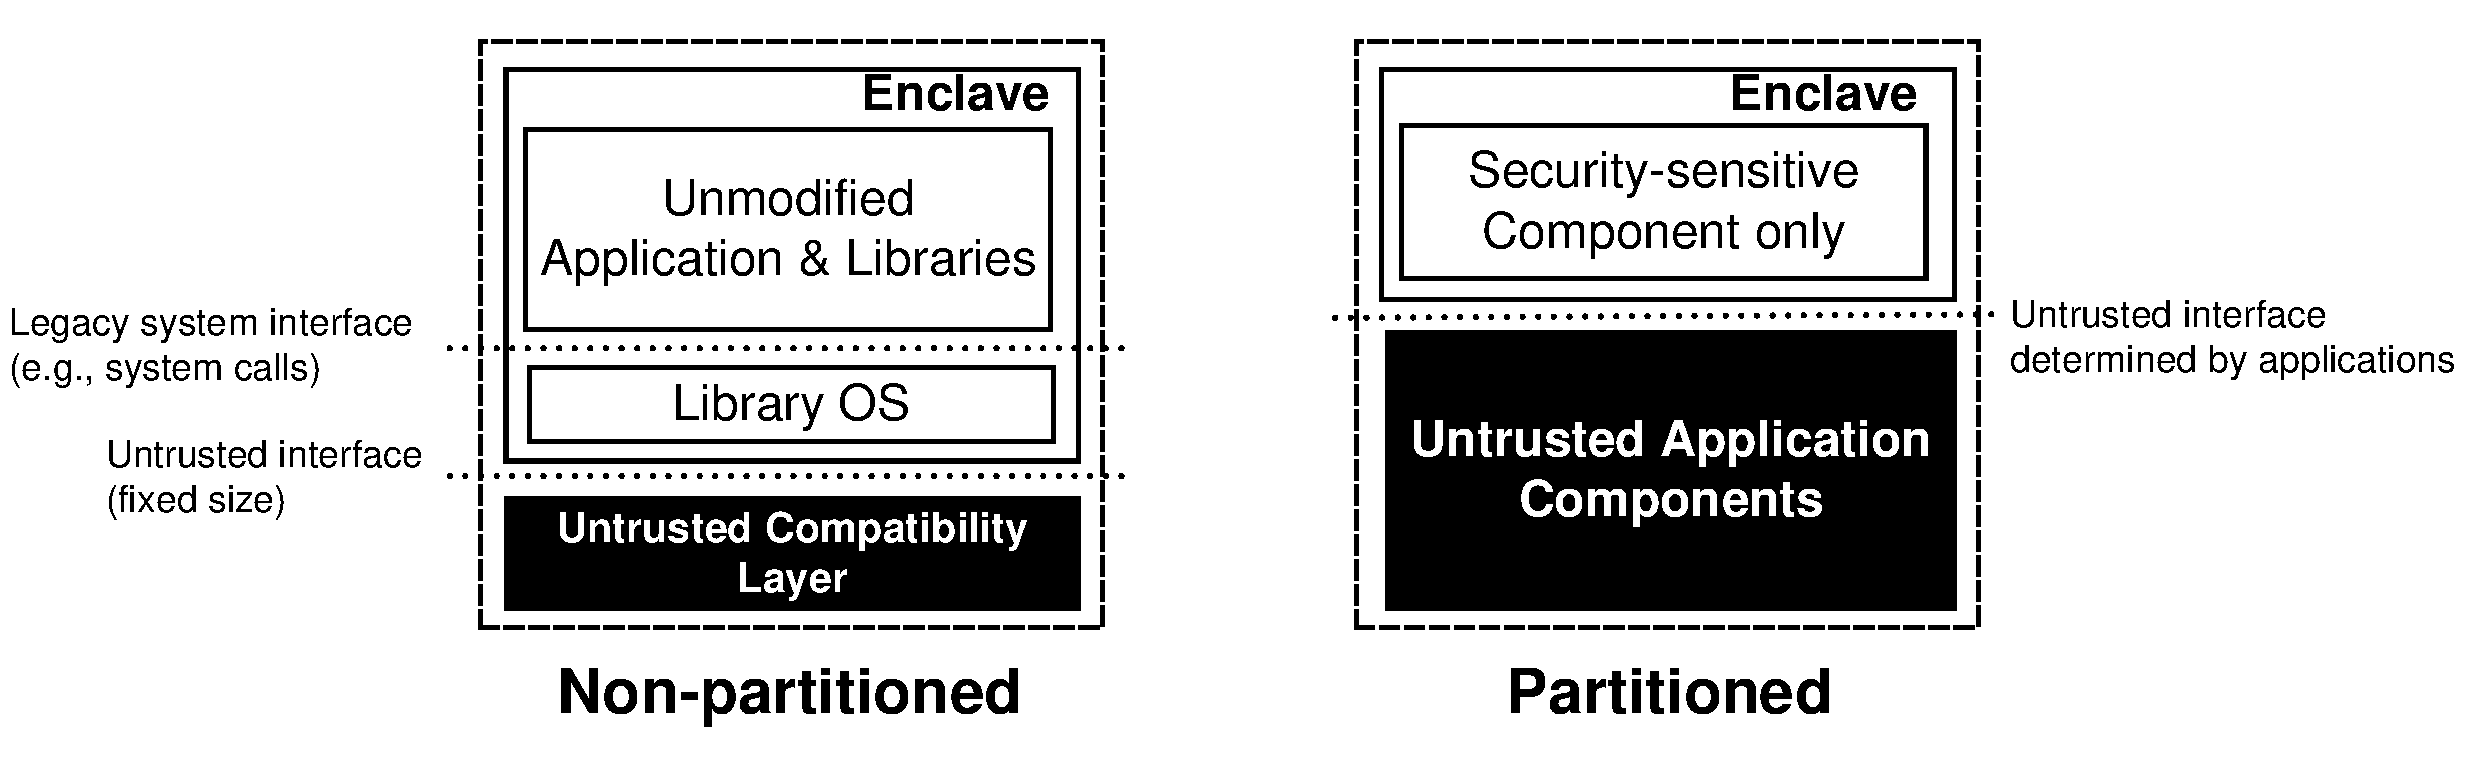
\includegraphics[width=6.5in]{graphene-sgx/figures/libosvssdk.pdf}
\vspace{-0.3in}
\caption[Comparison between two usage models of \sgx{}.]
{Comparison between the Non-partitioned model (e.g., Haven)
and partitioned model for protecting applications in enclaves.
Green (light) boxes are trusted components and red (dark) boxes are untrusted.
The non-partitioned model yields a larger TCB in the enclave,
while the partitioned model requires developers to determine the untrusted interface at the enclave boundary.}
\label{fig:civet:libosvssdk}
\end{figure}

\subsection{Challenges in Partitioning \java{} Applications on \sgx{}}

Using a higher-level language can be useful to reduce the risk of semantic errors in an application,
yet there are several fundamental, technical challenges to using a managed language, like Java,
in an SGX enclave.
In part, this is simply an artifact of the SGX design, which is designed
for native libraries.
To our knowledge, no previous work has successfully executed a JVM inside an enclave.

%% For developers who prefer implementing applications in a higher-level language like \java{} ---
%% to limit the vulnerabilities in the applicatins,
%% and use the partitioned model to protect the applications with \sgx{}
%% --- to reduce the TCB of enclaves,
%% the combination of two protections can be challenging.
%% For starter, \sgx{} enclaves are not designed to run any applications that are not native binaries.
%% Even though using the non-partitioned model with a library OS like Haven
%% can potentially run \java{} applications with the whole \java{} VM
%% inside the enclaves,
%% the technical effort required is non-trivial,
%% and no previous work has demonstrated any successful case yet.
  
%% \paragraph{Introducing \sgx{} to \java{}.}
%% We identity several challenges in presenting the \sgx{} protection to
%% \java{} applications, to allow them to isolate their security-sensitive components.
%% The challenges are in fact more than just the technical efforts
%% to design a wrapper API for \sgx{} instructions.
%% The fundamental gap between the requirement of using \sgx{} enclaves
%% and the characteristics of the \java{} language
%% is the primary pitfalls in combining them.
%% The requirements are not limited to \java{} and \sgx{},
%% but can apply to other languages and hardware protections.
%% \fixme{The discussion of the three primary problems must match section~\ref{sec:concept}.} 


%%% \sgx{} enclaves provide strong isolation guarantee for applications,
%%% against the malicious or vulnerable application components, system stack,
%%% and hardware (except the CPU itself).
%%% However, the security guarantees of the \sgx{} enclave is dependent on whether the developers design perfect applications without exploitable vulnerabilities that may compromise the application's security.
%%% As the application developers are not perfect,
%%% even applications or components isolated in enclave can face threats to their security.
%%% As follows, we discuss a few potential threats
%%% to the enclave security,
%%% even under the assumption that the SGX hardware is implemented as completely secure --- which can be another threat otherwise. 

%\fixmedp{I roughly want the rest of this section to have a problem, explanation, solution structure, with the overall theme being that this is subtle and we really need some analysis tools to get this right}


%% \paragraph{Applications are not perfect} 
%% The \sgx{} hardware cannot prevent applications from copying secrets out of the enclave without limiting functionality.
%% The trusted isolated components can copy any sensitive data from the enclave to the unencrypted memory, and potentially leak the enclave secrets.
%% The primary risk in the isolated components
%% is often memory corruption vulnerabilities, such as buffer overflow,
%% %Because in enclave applications can access any part of out-of-enclave memory unrestrictedly,
%% prevalent in applications that are not implemented in type-safe languages.

%% The best known technique to prevent vulnerabilities is to model the applications and verify them using {\em formal verification}.
%% While Sinha et.al.,~\citep{moat} use formal verification to prove confidentiality of enclave programs, it is impractical to accurately model complex sophisticated applications.
%% As a result, in addition to formal verification, maintaining smallest TCB
%% in the isolated components is the most practical approach 
%% to ensure enclave security,
%% and is the main reason to choose partitioned programming model over
%% libOS-based model.


%\begin{figure}[t!]
%\centering
%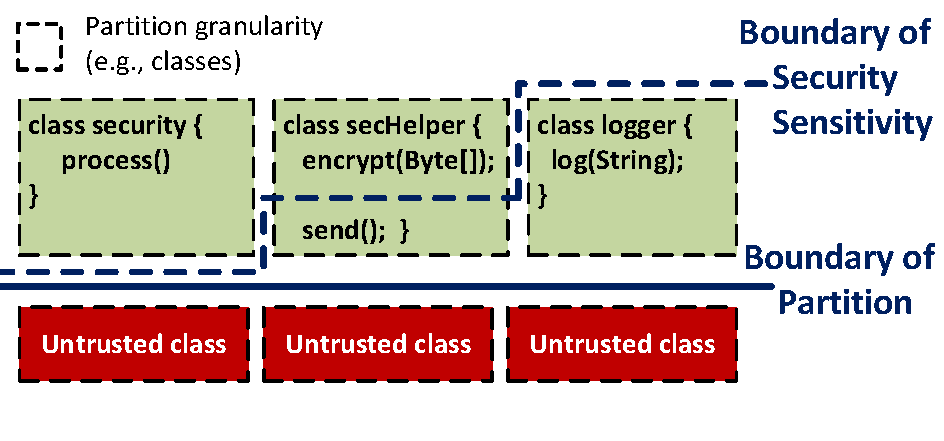
\includegraphics[width=\linewidth]{figures/partition.pdf}
%\footnotesize
%\vspace{-0.3in}
%\caption{
%Partitioning --- either manually or by automated tool ---
%often causes wider boundary of partition than the actual security sensitivity boundary
%due to (a) design granularity : {\tt SecHelper} contains a {\tt send()} method that is not partitioned from the rest of the class by design.
%or (b) better performance :  the less security sensitive {\tt logger} class is kept in 
%the privileged level to service frequent method calls. \fixmebj{Initial letter of all 
%class names must be Capital.}
%}
%\label{fig:partition}
%\end{figure}

%However, even if developers partition the applications and run only
%security sensitive components in the enclave,
%the developers may still leave some code irrelevant to
%enclave secrets inside the enclave.
%The reasons of having more-than-minimal TCB in enclaves
%are often that developers have to partition code in the granularity of source files or functions,
%or developers have to import more code to limit the width of interface and
%the frequency of interaction with the untrusted code.


\paragraph{\bf Challenge 1: Cleanly partitioning classes and objects (\S\ref{sec:civet:concept:partition}).}
Java encapsulates the placement of object data and code within virtual memory, which facilitates features
like inheritance and garbage collection, but complicates integration with SGX.
To program for an \sgx{} enclave, the developer must understand which regions of virtual memory 
are in the enclave, and which are outside of the enclave.
Note that \sgx{} allows code in the enclave to access memory
outside of the enclave.  Thus, it is easy for a developer to inadvertently write
code that discloses a secret, say by using a library that memoizes intermediate results to the untrusted heap.
Further, when a Java class inside of an enclave inherits methods or fields
from a parent class that is placed outside of the enclave, it is easy to 
inadvertently pass sensitive inputs to a function outside of the enclave,
or update a class field outside of the enclave.

In order for programmers to be able to sensibly program for SGX, they need
a model of how objects are placed inside and outside of the enclave at runtime, and as well as a model
for if and when updates to objects are propagated across the enclave boundary.
%% \sgx{} enclaves isolate the trusted components from the rest of the application,
%% and makes sure that no code or data
%% is shared between the trusted and untrusted parts.
%% For languages like C, which statically define functions and variables, it is easier for developers to cleanly
%% draw the line between trusted and untrusted components.
%% However, for a managed language like \java{}, a class can be inherited by other classes,
%% or referenced as other classes's fields, so the class may belong to both
%% untrusted and trusted components.
%% As a result, developers may struggle to manually partition the \java{} classes, especially if large portions of the classes are imported from libraries and not written by themselves.

%Reasoning about where in a program to draw the line between 
%trusted and untrusted code is subtle.
%On one hand, the developer has an incentive to minimize the size of the 
%API between the enclave and untrusted code, as well as an incentive to
%minimize the total code in the enclave.  These goals can sometimes be at odds.
%Each entry and exit to an enclave has a cost roughly comparable to a
%process context switch\fixmedp{right?}; an easy way to reduce enclave entries and exits is to simply 
%pull more code into the enclave, which increases the size of the TCB. For instance, in Figure~\ref{fig:partition}, even if the class {\tt Logger} is not security sensitive, 
%it is included in the enclave side of boundary of partition to avoid frequent entries and exits out of enclave.


%\fixmedp{I'm not sure how to explain Figure~\ref{fig:partition}, but it needs an explanation.}

%Fundamentally, the art of paritioning an application is to find a ``pinch point'' or
%``narrow waist'' in the application, where there is a natural point to insert an API and 
%security checks.  This is indeed as much art as science, often done manually by experts\fixmedp{any more supporting evidence or cites?}. Moreover, different classes of applications in managed languages like \java{} are tightly coupled; and it is necessary  to widen the boundary of partition to include some non-sensitive code in the trusted component.
%For instance, in Figure~\ref{fig:partition}, even if the {\tt send()} method is not security sensitive, it has to be included in the enclave code because of the design of the class {\tt SecHelper} to achieve a clean partition of the application.
%It is unlikely that the average developer will successfully navigate this design process without analysis tools, such as \fixmedp{examples?},
%to help identify these natural division points.


%% Experts can use a manual partitioning technique to achieve smallest TCB for the isolated components compared to automated tools.
%% However, the manual partitioning costs a lot of effort,
%% and rare expertise, lack of which can cause larger TCB.

%% Neither manual nor automated partitioning is perfect:
%% the resulted boundary of partitioning often has a gap from the actual boundary of security sensitivity (as shown in figure~\ref{fig:partition}),
%% leaving more code in the privileged level
%% than what's actually needed.
%% Having the gap between the ideal and resulted boundary
%% is mostly inevitable, due to multiple reasons.
%% One common reason is the granularity of partitioning,
%% which can vary from a binary file, a component, a source file,
%% a class, a method (a function) to a line of code.
%% Another reason is that a component or a method may be too frequently called
%% by the security sensitive code,
%% laying the boundary between the component or method from the security sensitive side may bring too much overhead or risk,
%% because the execution crosses the boundary too often.
%% Therefore, developers often will balance among the effort of partitioning,
%% risk or cost of communicating between different partitions,
%% and minimizing the TCB in the security sensitive parts.

%\fixmedp{Maybe move the commented paragraph below down into the design section?  I'd like to downplay the plugs for our work here, and instead fulfill these promises later}
%% \sysname{} automates partitioning of applications,
%% based on the boundary at the classes which the developers marked
%% as the interfaces of the enclave.
%% Only the classes that are depended by the marked classes
%% will be included in the enclaves,
%% to minimize the TCB.
%% Although not all classes pulled into the enclaves
%% are necessarily security sensitive,
%% the enclaves are protected from the potential vulnerabilities in those classes,
%% by the security guarantees of \java{} language,
%% and the information flow tracking in \sysname{}.

%Another threat to \sgx{} is the vulnerability of the 
%security sensitive code running in the Enclave. The 
%main guarantee of \sgx{} to isolate the secure data 
%from other components and privileged OS is undermined 
%if the Enclave code can be tricked to leak the 
%security sensitive data to the attacker. Executing 
%buggy code in \sgx{} enclave can inadvertently leak 
%information if the attacker can exploit memory-safety 
%vulnerabilities like buffer overflow and dangling 
%pointers.  

% Cumbersome and approximation to partition code
%The developers have to manually partition their code 
%into security sensitive and insensitive part. If this 
%partitioning is done by a novice developer, some of 
%the security insensitive parts of the application can 
%end up in the security sensitive part, increasing the 
%Trusted Computing Base(TCB). Moreover, the 
%partitioning of code is not straightforward, which 
%can also contribute to a less stricter TCB. The bigger the TCB, the more %vulnerable is the Enclave code to attacks.

% Buggy Code leads to inadvertant information leakage


% SGX code only Integrity protected not confidential
%Moreover, \sgx{} only protects the integrity of the enclave code. The security critical part of the application is stored in plaintext while the secret data is provisioned securely after attestation. However, \sgx{} does not protect the confidentiality of enclave application code which may be executing a secret algorithm. \fixmebj{Talk more about the problem motivating security tag preservation.}
%\sgx{} can natively guarantee either code integrity or
%code confidentiality (as part of the enclave data), but not both.
%If application code is included in the enclave measurement and
%verified by the hardware,
%the code must stay in plaintext as part of the enclave image.
%If any code is stored or provisioned in encrypted forms,
%the application or infrastructure in enclave must dynamically load
%the code after decryption.
%Supporting dynamic loading makes enclaves open to code injection
%if the applications have exploitable vulnerabilities.

\paragraph{\bf Challenge 2: Dynamically loading byte-code with integrity (\S\ref{sec:civet:concept:loading}).}
\sgx{} establishes trust by verifying the integrity of the code in the enclave.
Therefore, enclaves must be bootstrapped with static, native binaries.
%that have consistent measurements.
However, \java{} classes are shipped as byte-code,
and dynamically loaded by \java{} VMs.
The subtle security challenge for a Java developer 
is ensuring that, when a class is dynamically loaded into an enclave, by passing a string name of the class,
the application needs to be able to verify that this is a trusted class file
and that the initial state of the class is correct.
Thus, we introduce techniques to manage trust and verify the integrity of 
dynamically loaded code, including encrypted class files.

%This means the SGX enclaves can only guarantee the code integrity of the initially loaded infrastructure, which in turn has to
%verify the integrity of classes dynamically loaded.
%\fixmedp{Can you say a bit more about why this is hard or interesting?}

%The hardware-level \sgx{} code integrity mechanism is based on a cryptographic
%signature of a static binary in plaintext.
%If any application dynamically loads any code after the enclave's initial measurement,
%the initial application must be trusted to attest the loaded code.
%The subtle tension is that there is no way to protect the confidentiality of
%a secret algorithm, except by dynamically loading an encrypted binary.
%Dynamically loading code increases the risk of code injection attacks and other control flow compromises. The interpreted and managed languages effectively compound the
%risks by dynamically loading all the application code.

%Any application partitioning solution that protects sensitive algorithms and data
%must have a robust dynamic loader that can measure encrypted libraries or classes.
%\sysname{} includes a loader that can measure encrypted class files,
%provisioned from a trusted host.

%% \sgx{} enclaves require code integrity in the isolated applications.
%% If the code integrity is not maintained, adversaries can corrupt the enclave code to
%% force the applications to leak the information provisioned from the remote,
%% trusted hosts.
%% \sgx{} hardware only guarantees
%% the integrity of the code initially loaded into the enclaves.
%% However, if an application choose to dynamically
%% load any code after the enclave starts,
%% the application is responsible for the integrity of the code loaded.
%% The fact that dynamic loading of applications, libraries or components
%% is a feature that can potentially make enclaves vulnerable and open to code injection,
%% raises concerns against supporting managed languages in the enclaves.

%% On the other hand, code confidentiality can be a desirable feature,
%% for application developers who prefer keeping the secret sauce of their algorithms concealed.
%% To enable the feature of code confidentiality in enclaves, the protected code must be dynamically loaded into the enclave,
%% because the \sgx{} hardware only accept
%% the initial loaded code to be in plaintext.
%% \sysname{} provides both code integrity and confidentiality by verifying
%% every classes dynamically loaded into the enclaves,
%% and allows loading classes provisioned from trusted hosts.


%% In general \sgx{} enclaves are prone to having side channels, such as timing channels. Because \sgx{} relies on the untrusted OS for paging,
%% an enclave will always leak page fault addresses, except the lower 12 bits (offsets in pages).
%% Such a leakage gives the untrusted OS to amplify the side channels,
%% by forcing page faults on every instruction or memory access.
%% This so-called {\em Controlled Channel Attack} is common to all applications who use \sgx{} protection, regardless of the programming models.
%% \sysname{} does not specifically defend against side channel attacks.

%% \paragraph{Denial-Of-Service Attacks}
%% \sgx{} is not designed to be safe against denial-of-service attacks.
%% Because the untrusted OS still controls the host resources,
%% there are countless ways to prevent an enclave from making progress.
%% For example, the OS can simply starve the enclaves by
%% never scheduling CPU, memory or other resources to the enclaves.
%% \sysname{} does not specifically defend against denial-of-service attacks.

\paragraph{\bf Challenge 3: Seamless access of in-enclave objects (\S\ref{sec:civet:concept:interface}).}
Java code outside of the enclave must be able to call enclave entry points and 
have some notion of objects that are inside the enclave.
Unlike C, where most function addresses are determined once and statically
at the dynamic linking phase,  Java identifies most functions through
object references (e.g., {\tt Foo.toString()}).
Thus, the untrusted code must be able to reference
objects inside of the enclave in a way that makes sense when
the untrusted code behaves correctly, but that does not create unexpected information flows 
out of the enclave.
Similarly, the developer needs a constructor interface to declare which dynamically-created
objects should be placed in the enclave and which should be outside of the enclave. 


%% For native binaries, enclave entry points are statically inserted
%% into the untrusted code
%% at explicit locations known to interact with the enclaves.
%% However, for \java{} applications, instantiating or calling methods
%% on isolated components must dynamically trigger enclave entry.
%% For instance, calling the {\tt toString()} method of any object 
%% may trigger enclave entry based on whether the object's reference type is in the enclave.
%% Moreover, the the objects and methods determine the entry targets (the locations where the execution transfer after entering the enclaves) and the arguments passed into the enclaves at entry.
%% Unlike native binaries, the code behavior at enclave entry must be determined at runtime.
%% \fixmedp{I don't understand this point yet.  Is the issue that the untrusted code needs to track
%% opaque references into the enclave?  Can you explain more?}


%The \sgx{} hardware ensures that the enclave only has fixed number of entry points 
%(exactly one location where the execution starts, but multiple pre-defined locations 
%that the execution can jump to). However, for an application written in a language like JAVA with a virtual machine or interpreter, there are no clear entry points separating 
%the trusted and untrusted components. Moreover, due to the approach of executing intermediate code, it is also difficult to determine the entry points at runtime.

%Just separating an application into parts based on security sensitiveness is not enough to securely isolate the two parts using \sgx{}. In addition to application partition, there is a need to automatically determine the entry points without offloading the effort to the developers. \sysname{}  automatically identifies and exports all untrusted interfaces to the isolated classes at build time.

%\paragraph{Discussion.}
%This section has outlined several pitfalls for developers of partitioned applications.
%These common pitfalls render the hardware protections of SGX useless.
%Language-level analysis can automate error-prone reasoning in the best case, or, in the worst case, 
%can at least offer invaluable guidance to the developer.  For SGX-style
%hardware to be useful to a wide array of developers, developers need language-level
%tools that can also factor in hardware-level protection mechanisms.

\begin{comment}

\subsection{The Challenges of Combining Language and Hardware Protections}

Language and hardware protections provide varying benefits
to application security:
Languages improve the internal security inside the applications,
while hardware provides the base defenses that cannot be easily overridden or bypassed.
Commonly security experts exploits both types of protections
to further harden the security of applications.
For example, hardware protections may take information from the language runtimes or compilers to enforce the security policies,
or language protections may rely on hardware protections to bootstrap the initial trust they need. 

However, the combination of language and hardware protections is more
like a trick of the trade for security experts:
the use of hardware protections is deeply buried in the design of language protections,
so that users (application developers) lose direct access
to the security guarantees and features provided by the hardware.
\fixme{Think of an example: Maybe TPM.}
The approaches of combining language and hardware protections are mostly ad-hoc to the use cases,
i.e., how one protection is used to improve or reinforce another.

There are two reasons for why combining language and hardware protections
is so inevitably hard.
First, hardware protections often have restrictions
on the languages that must be used
to access the security guarantees and features of the hardware.
For example, \sgx{} requires the loaded code to be implemented in C or C++,
or any languages that can compile applications into static binaries.
The restriction is not simply a design decision
made by the hardware or its SDK,
but a result of the fact that SGX requires a static image to guarantee the integrity of execution.
On the other hand, if the language used is a managed language like \java{},
accessing SGX hardware will be cumbersome,
because it is hard to provide any APIs to allow direct access to the SGX hardware,
to harvest its security guarantees
or to utilize its features.

\begin{figure}[t!]
\centering
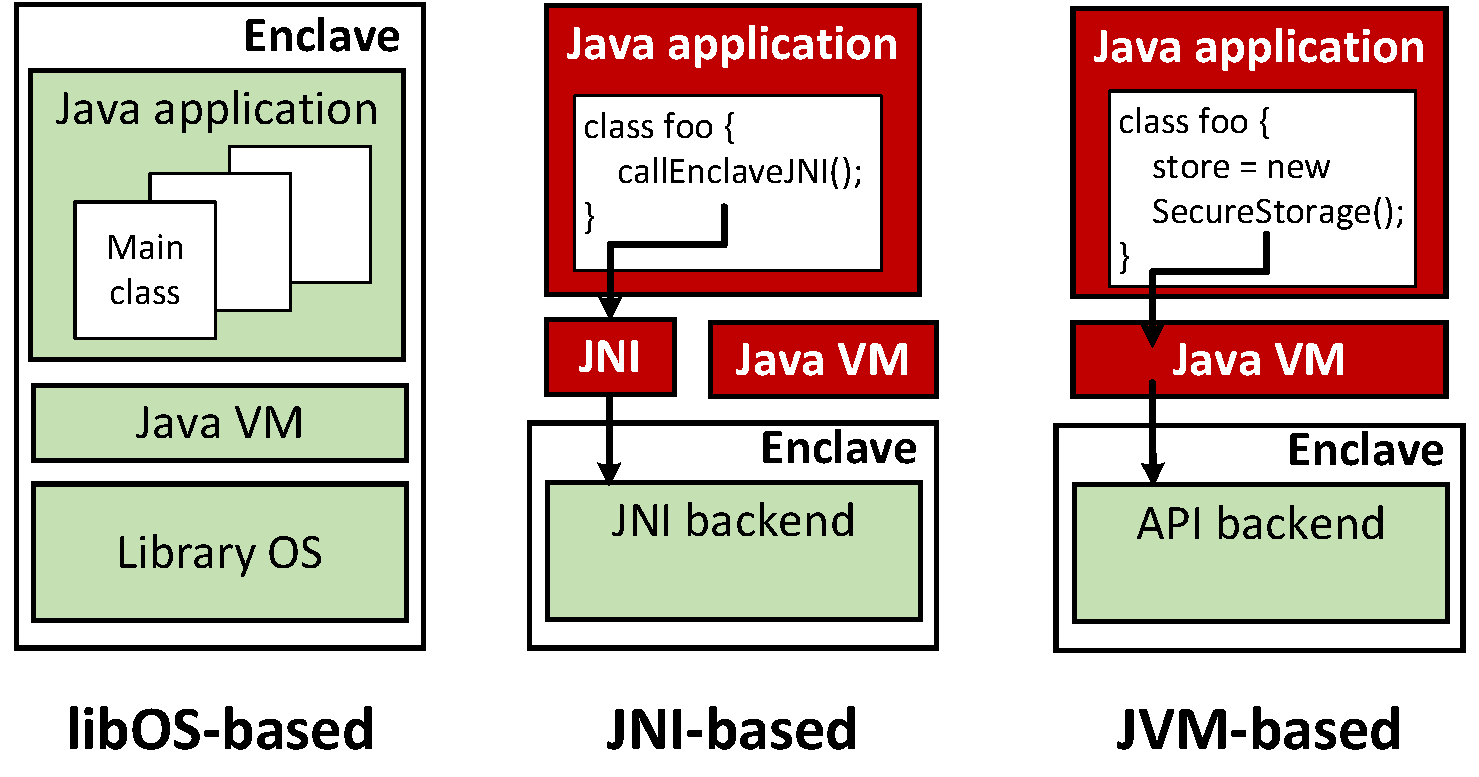
\includegraphics[width=\linewidth]{civet/figures/alternatives.pdf}
\footnotesize
\caption{Alternative approaches to access \sgx{} hardware protection from \java{} applications.
The {\em libOS-based} approach runs the whole \java{} applications in the enclaves. 
The {\em JNI-based} approach uses JNI to run the security sensitive operations inside the enclaves.
The {\em JVM-based} approach requires the \java{} VM to provide APIs to support common use cases of the enclaves.
Green (light) boxes are trusted components and red (dark) boxes are untrusted.
}
\label{fig:civet:alternatives}
\end{figure}


Figure~\ref{fig:civet:alternatives} illustrates the alternative approaches
to access SGX hardware from \java{} applications:
The first approach is to run the whole \java{} applications with the \java{} VM inside the enclaves,
using a library OS ({\em libOS-based}).
This approach can secure applications as a whole,
but won't support any partitioned model for programming.
Another approach is to implement a JNI that create and interface with the enclaves
to run the security-sensitive operations ({\em JNI-based}).
The JNI-based approach is flexible enough for application developers
to implement the isolated components as well as the untrusted interface,
but requires developers to have the knowledge of
enclave implementation.
More importantly, the isolated components can only be developed in C or C++
language, so the applications lose the language protection of \java{} inside the enclaves.
A more plausible approach is to provide enclave-backed APIs
from the \java{} VM,
to support common use cases ({\em JVM-based})), such as a secure key-value store~\citep{vc3}.
Although the JVM-based approach can save the application developers' effort
of implementing isolated components,
the use cases is limited to the pre-defined operations provided by the \java{} VM or the companion frameworks.
Because the backend implementation (isolated components and untrusted interfaces) in the JVM-based approach is the same as the JNI-based approach,
the same language restriction also applies here. 

\end{comment}

%- Motivate the problem.
%- List all attack vectors
%- How can JAVA help?

\paragraph{Discussion.}
Partitioning an application requires some input from the developer in order to identify 
sensitive data and code.  Each of the challenges above highlight cases where
Java either hides important information from the developer, or otherwise useful runtime
techniques can thwart the isolation benefits of using a hardware mechanism like SGX.
A higher-level goal of \sysname{} is to provide constructs for the developer to specify
her goals, such as which objects should be isolated in an enclave,
and to have the language runtime use these developer-provided hints to 
make judicious choices on issues such as data placement.
A related goal is not eroding the benefits of developing in a high-level, managed language runtime.


%% The combination of language and hardware protections
%% is a technique used by many previous works.
%% However, the approach often seems like a trick of the trade for security experts:
%% the use of hardware protections is often deeply buried in the design of language protections,
%% as the underlying mechanism to bootstrap the trust
%% or to secure the core components of language protections.
%% %so that users (application developers) lose direct access
%% %to the security guarantees and features provided by the hardware.
%% %\fixme{Think of an example: Maybe TPM.}
%% %The approaches of combining language and hardware protections are mostly ad-hoc to the use cases,
%% %i.e., how one protection is used to improve or reinforce another.
%% This work chooses a different approach,
%% by allowing \java{} applications
%% to straightforwardly utilize the protection of \sgx{} enclaves,
%% while still benefit from the safety properties
%% and advanced language protections from \java{}.
%% As a result, our framework also opens the win-win opportunity for
%% hardening both \sgx{} and \java{} protections.
%% \fixmedp{I also don't understand the point of this discussion.  What do you want the reader to learn from this?}
